\section{Numerical Method for Shear flow}
\begin{frame}
	\scriptsize
	We rewrite the time-dependent Smoluchowski equation as a system of inhomogeneous conservation laws
	\begin{align}
		\partial_t Q(x,t) + \textcolor{blue}{A}\partial_x Q(x,t) = \textcolor{red}{\varphi} (Q(x,t)),
	\end{align}
	where $Q(x,t) = (f_0, c^{-2}_2, c^{-1}_2, ..., c^2_2)$ is. \\
	\vspace{0.5cm}
	Solve this problem by splitting it into two subproblems of the form
	\begin{enumerate}
		\item $\partial_t Q(x,t)  = \varphi (Q(x,t))$
		\item $\partial_t Q(x,t) + A Q_x=0$.
	\end{enumerate}
\end{frame}

\begin{frame}
	\scriptsize
	\begin{enumerate}
		\item Drift diffusion term
		\begin{equation*}
			\partial_t \left(\begin{array}{c}
				f_0 \\
				c_2^{-2} \\
				c_2^{-1} \\
				c_2^0 \\
				c_2^1 \\
				c_2^2
			\end{array}\right)  = \begin{pmatrix}
				0 & 0 & 0 & 0 & 0 & 0 \\
				0 & -6D_r & \frac{2}{7}w_x & 0 & 0 & 0 \\
				-\frac{\sqrt{15}}{5}w_x & -\frac{5}{7}w_x & -6D_r & \frac{3\sqrt{3}}{7}w_x & 0 & 0 \\
				0 & 0 & -\frac{4\sqrt{3}}{7}w_x & -6D_r & 0 & 0 \\
				0 & 0 & 0 & 0 & -6D_r & -\frac{5}{7} w_x\\
				0 & 0 & 0 & 0 & \frac{2}{7}w_x & -6D_r
			\end{pmatrix} \cdot
			\left(\begin{array}{c}
				0 \\
				c^{-2}_2(t) \\
				c_2^{-1}(t) \\
				c_2^0(t) \\
				c_2^1(t) \\
				c_2^2(t)
			\end{array}\right).
		\end{equation*}
	\item Solve the advection equation
		$$
	\partial_t \left(\begin{array}{c}
		f_0 \\
		c_2^{-2} \\
		c_2^{-1} \\
		c_2^0 \\
		c_2^1 \\
		c_2^2
	\end{array}\right) + \begin{pmatrix}
		0 & 0 & \frac{\sqrt{15}}{15} & 0 & 0 & 0 \\
		0 & 0 & \frac{1}{7} & 0 & 0 & 0 \\
		\frac{\sqrt{15}}{15} & \frac{1}{7} & 0 & \frac{\sqrt{3}}{21} & 0 &  0 \\
		0 & 0 & \frac{\sqrt{3}}{21} & 0 & 0 & 0 \\
		0 & 0 & 0 & 0 & 0 & \frac{1}{7}\\
		0 & 0 & 0 & 0 & \frac{1}{7} & 0
	\end{pmatrix} \partial_x \left(\begin{array}{c}
		f_0 \\
		c_2^{-2} \\
		c_2^{-1} \\
		c_2^0 \\
		c_2^1 \\
		c_2^2
	\end{array}\right) = 0
	$$
	with one-dimensional resolution Wave Propagation Algorithm
	\end{enumerate}
\end{frame}

\begin{frame}
	\scriptsize
	Consider a Riemann Problem for externally imposed shear flow with $wx/D_r = 0.5$ for the left state and $wx/D_r = 1$ for the right state.
	\begin{figure}[H]
		\centering
		\begin{minipage}{0.32\textwidth}
			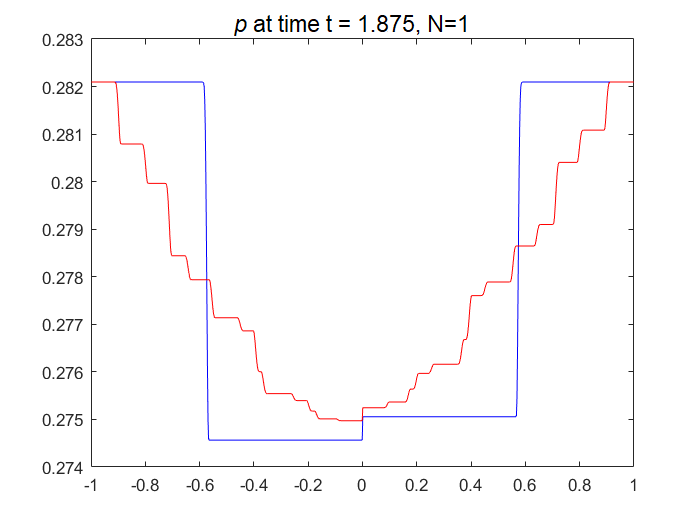
\includegraphics[width=\textwidth]{Bilder_wx/Wavepropa/red=12th_blue=2nd_wx=1_leftDr1_rightDr2_Awp12th}
		\end{minipage}
		\hfill
		\begin{minipage}{0.32\textwidth}
			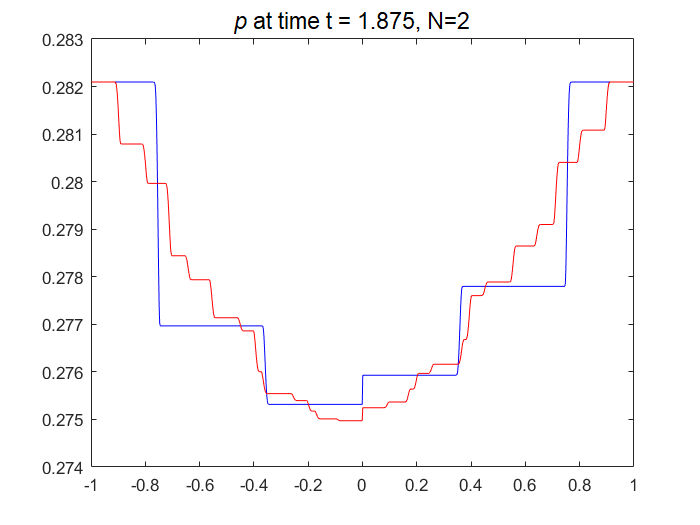
\includegraphics[width=\textwidth]{Bilder_wx/Wavepropa/red=12th_blue=4th_wx=1_leftDr1_rightDr2_Awp12th}
		\end{minipage}
		\hfill
		\begin{minipage}{0.32\textwidth}
			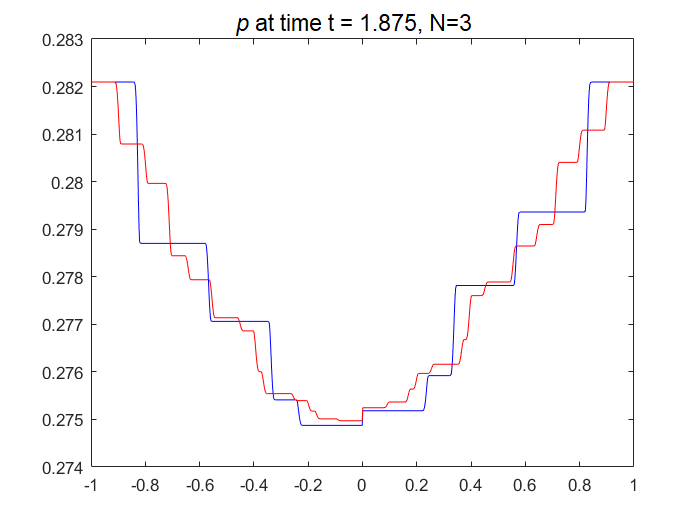
\includegraphics[width=\textwidth]{Bilder_wx/Wavepropa/red=12th_blue=6th_wx=1_leftDr1_rightDr2_Awp12th}
		\end{minipage}
		\vfill
		\begin{minipage}{0.32\textwidth}
			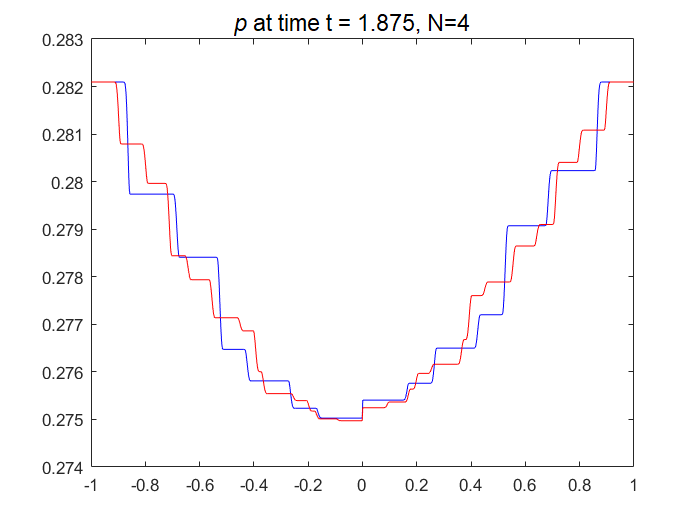
\includegraphics[width=\textwidth]{Bilder_wx/Wavepropa/red=12th_blue=8th_wx=1_leftDr1_rightDr2_Awp12th}
		\end{minipage}
		\hfill
		\begin{minipage}{0.32\textwidth}
			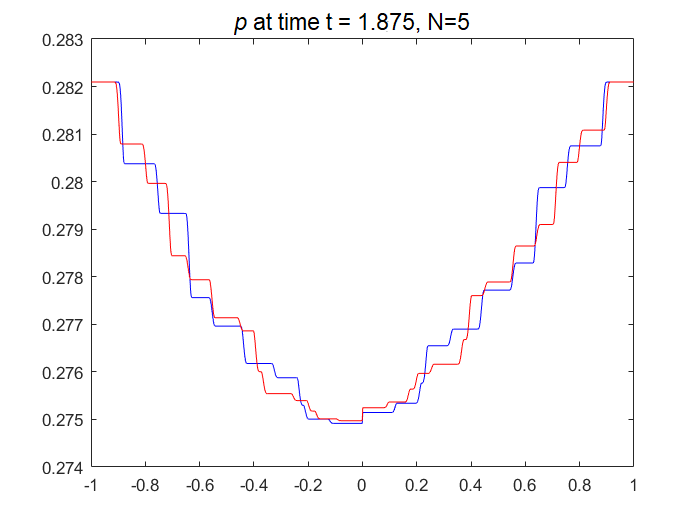
\includegraphics[width=\textwidth]{Bilder_wx/Wavepropa/red=12th_blue=10th_wx=1_leftDr1_rightDr2_Awp12th}
		\end{minipage}
		\hfill
		\begin{minipage}{0.3\textwidth}
			% Optional: Leave empty or add another image
		\end{minipage}
	\end{figure}
\end{frame}
